% Auto-generated by presentation_results_builder.ipynb

\begin{frame}{2.4 Alpha signal}
\begin{block}{Construction}
Synthetic short-horizon alpha with $H=5$m and $\rho=0.10$:
\[
\alpha_t^{bps} \approx 10^4\mathbb{E}\left[\frac{S_{t+H}-S_t}{S_t}\mid \mathcal F_t\right].
\]
\end{block}
\begin{columns}[T]
\column{0.48\textwidth}
\begin{itemize}
  \item Positive out-of-sample predictive content.
  \item Trades align with alpha direction.
  \item Gross alpha capture is positive before impact costs.
\end{itemize}
\column{0.52\textwidth}
\scriptsize% Pair 1 alpha diagnostics
\begin{tabular}{ll}
\hline
Metric & Value \\
\hline
$\mu(\alpha)$ bps & 0.001 \\
$\sigma(\alpha)$ bps & 0.232 \\
$\rho(\alpha,r_{t+H})$ & 0.190 \\
$\rho(q,\alpha)$ & 0.490 \\
$\rho(Q^+,\alpha)$ & 0.592 \\
$\Pr[\operatorname{sign}(q)=\operatorname{sign}(\alpha)]$ & 0.858 \\
Gross alpha ($m) & 33.02 \\
\hline
\end{tabular}

\end{columns}
\end{frame}

\begin{frame}{2.5 OW transient proxy strategy}
\begin{block}{Local proxy objective}
\[
\max_{q_t}\; q_t\alpha_t - \kappa_t q_t^2 - \gamma(Q_{t^-}+q_t)^2
\]
\end{block}
\begin{columns}[T]
\column{0.48\textwidth}
\begin{itemize}
  \item Reportable strategy: \texttt{OW\_transient\_proxy}.
  \item Participation cap: $|q_t|\leq 1\%$ volume.
  \item Inventory cap: $|Q_t|\leq 5\%$ ADV.
\end{itemize}
\column{0.52\textwidth}
\scriptsize% Pair 1 baseline detail, fitted proxy PnL
\begin{tabular}{ll}
\hline
Metric & Value \\
\hline
Gross PnL & 33.02 $m \\
Fitted proxy cost & 0.50 $m \\
Net PnL & 32.52 $m \\
Daily Sharpe & 1.88 \\
Max drawdown & -1.67 $m \\
Mean participation & 0.02\% \\
\hline
\end{tabular}

\end{columns}
\end{frame}

\begin{frame}{2.5 OW proxy wealth: pair 1}
\begin{center}
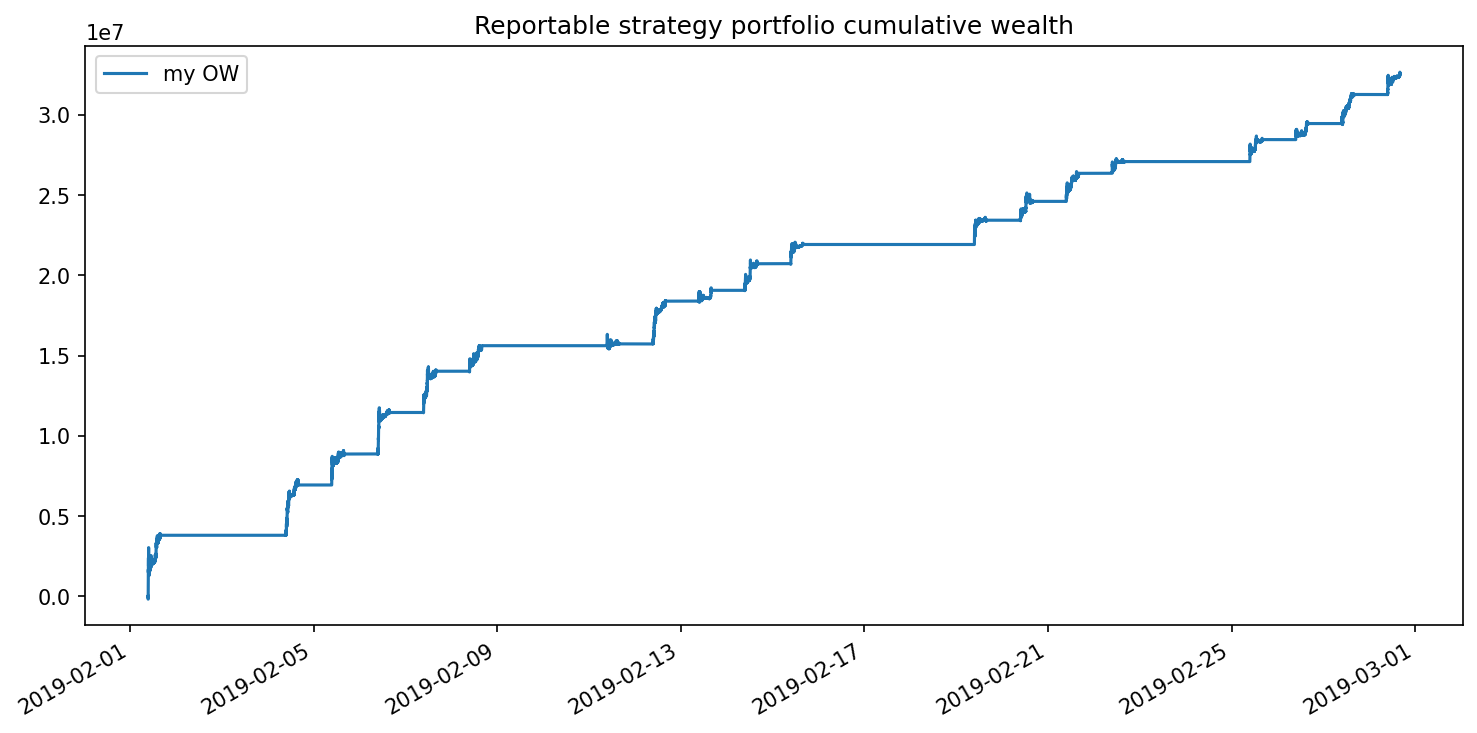
\includegraphics[width=0.88\textwidth]{outputs/presentation_assets/figures/ow_proxy_wealth_pair1.png}
\end{center}
\end{frame}

\begin{frame}{2.5 Baseline all-pairs results}
\begin{columns}[T]
\column{0.42\textwidth}
\scriptsize% Aggregate baseline statistics
\begin{tabular}{ll}
\hline
Statistic & Value \\
\hline
Mean net PnL & 48.87 $m \\
Median net PnL & 38.85 $m \\
Min net PnL & 28.15 $m \\
Max net PnL & 105.00 $m \\
Mean Sharpe & 2.27 \\
Mean max drawdown & -0.86 $m \\
Total net PnL & 537.57 $m \\
\hline
\end{tabular}

\column{0.58\textwidth}
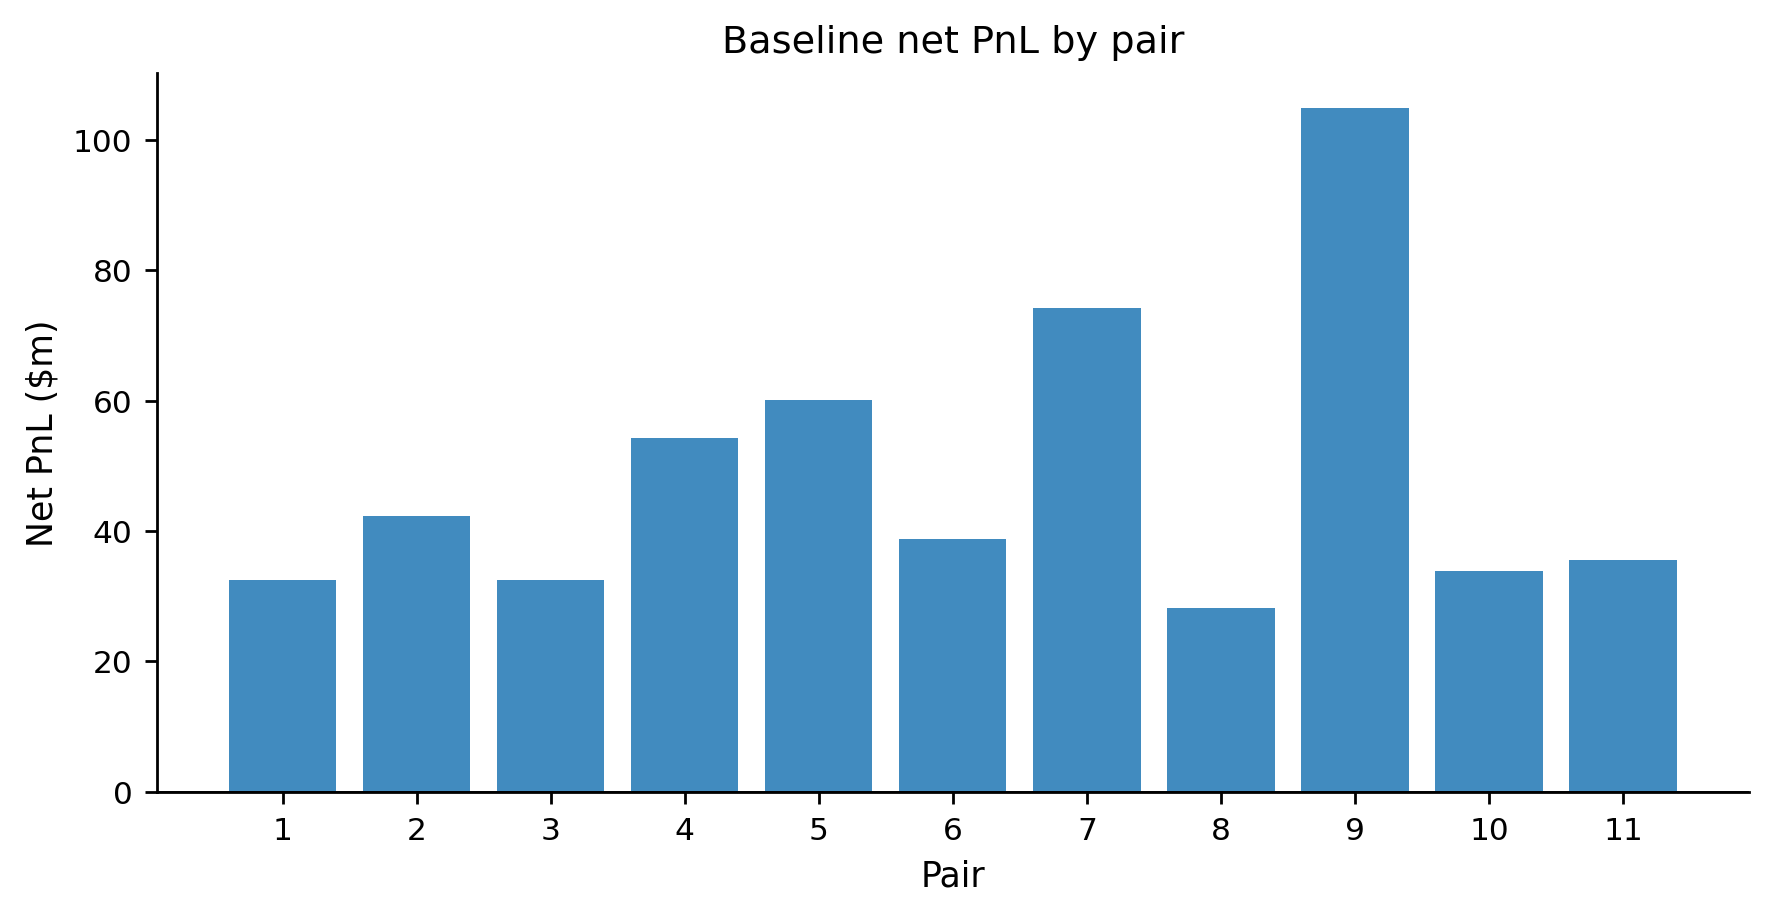
\includegraphics[width=\textwidth]{outputs/presentation_assets/figures/baseline_net_pnl_by_pair.png}
\vspace{0.1cm}
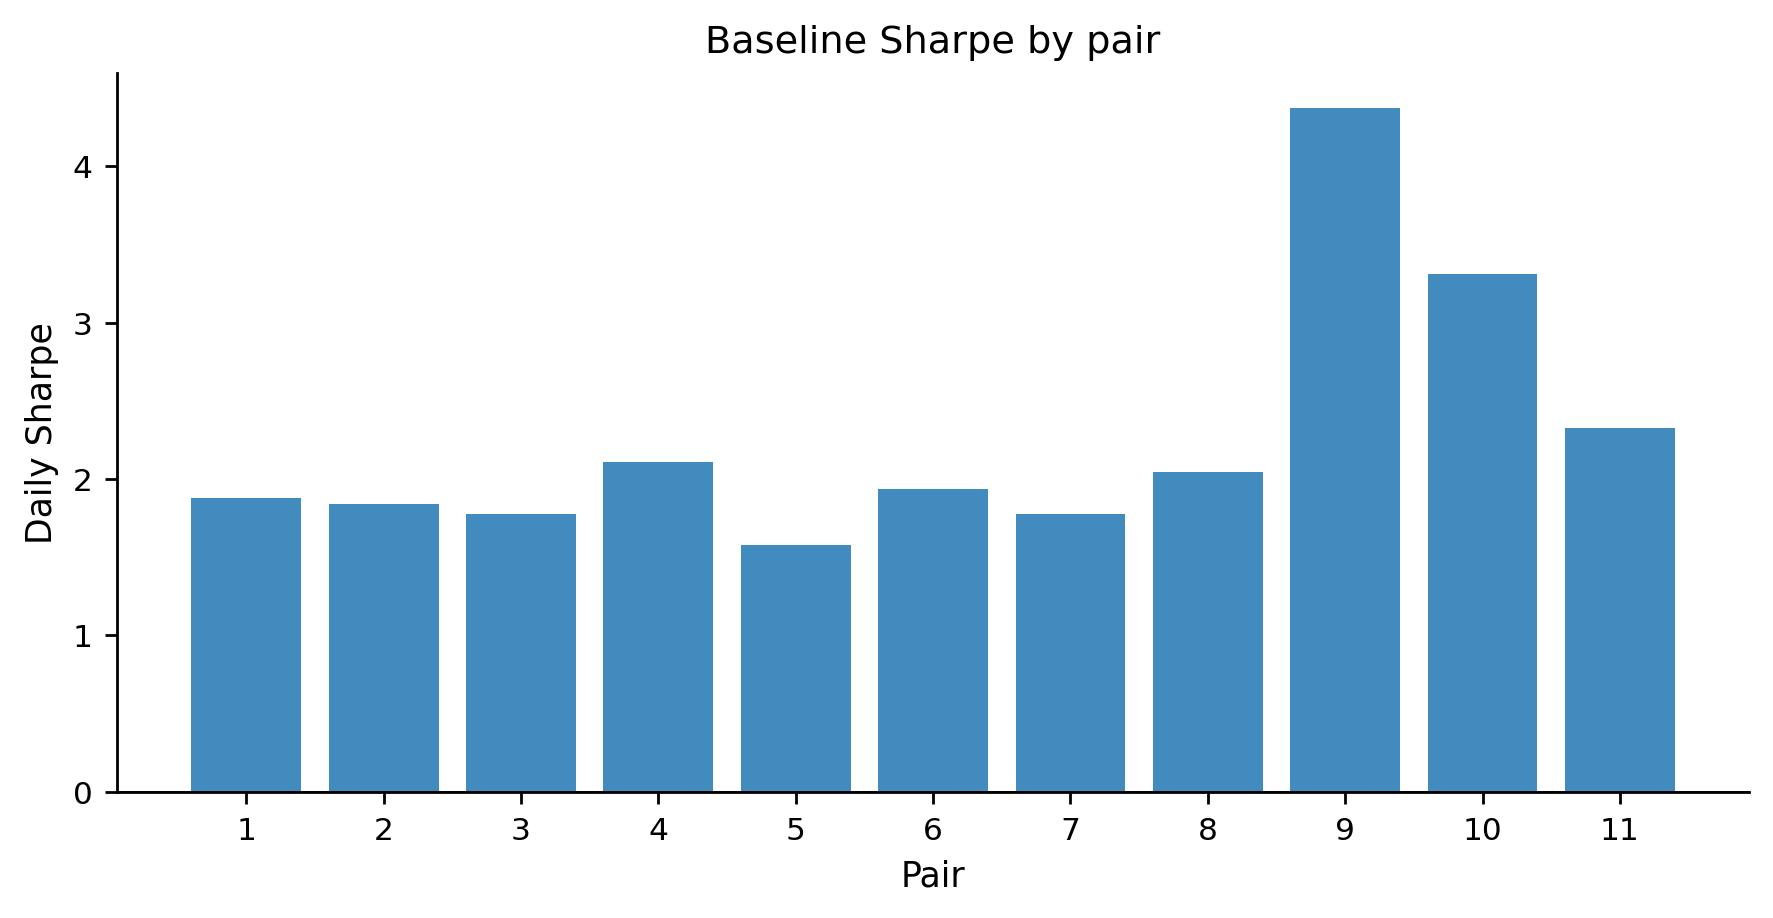
\includegraphics[width=\textwidth]{outputs/presentation_assets/figures/baseline_sharpe_by_pair.png}
\end{columns}
\end{frame}

\begin{frame}{2.5 Reduced-form proxy and model comparison}
\begin{block}{Same proxy, richer slope}
Reduced-form proxy uses the same myopic quadratic mechanism with marginal impact slope from the richer regression specification.
\end{block}
\begin{columns}[T]
\column{0.48\textwidth}
\begin{itemize}
  \item Compare model-consistent baselines against misspecified strategy paths.
  \item Correct RF: RF proxy under RF evaluator.
  \item Correct OW: OW proxy under OW evaluator.
\end{itemize}
\column{0.52\textwidth}
\scriptsize% Pair 1 net PnL ($m)
\begin{tabular}{lll}
\hline
Assumed strategy & OW eval & RF eval \\
\hline
OW proxy & 32.40 & 32.35 \\
RF proxy & 30.04 & 30.34 \\
\hline
\end{tabular}

\end{columns}
\end{frame}

\begin{frame}{Stress test: wrong model}
\begin{columns}[T]
\column{0.50\textwidth}
\scriptsize% Wrong-model loss = wrong strategy PnL - correct strategy PnL
\begin{tabular}{rlll}
\hline
Pair & Loss RF-true ($m) & Loss OW-true ($m) & RF-OW diff. ($m) \\
\hline
1 & 2.01 & -2.36 & -2.06 \\
2 & 0.48 & -0.97 & -0.68 \\
3 & -1.50 & -0.62 & 1.40 \\
4 & -0.90 & 0.31 & 1.15 \\
5 & -9.80 & 9.39 & 10.17 \\
6 & -0.64 & -0.74 & 0.44 \\
7 & 24.16 & -24.49 & -24.46 \\
8 & -0.84 & 0.45 & 1.19 \\
9 & 53.67 & -57.15 & -54.75 \\
10 & 1.00 & -2.54 & -0.65 \\
11 & -2.41 & -0.69 & 3.61 \\
\hline
\end{tabular}

\column{0.50\textwidth}
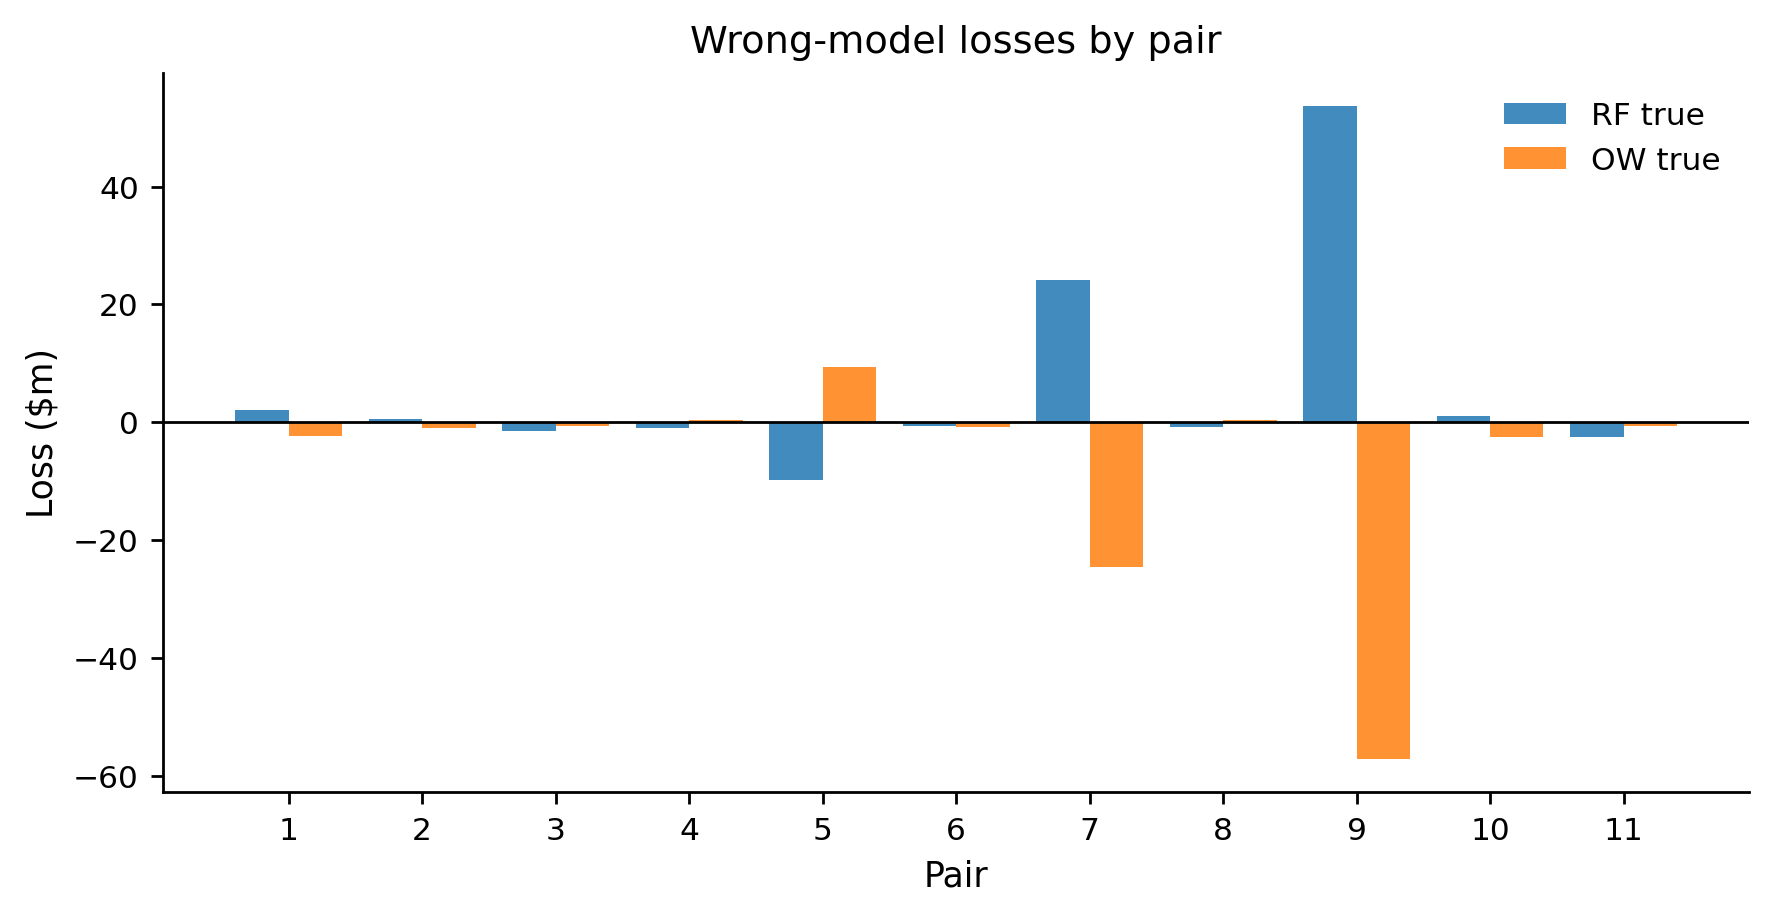
\includegraphics[width=\textwidth]{outputs/presentation_assets/figures/wrong_model_losses_by_pair.png}
\end{columns}
\vspace{0.2cm}
\small Misspecification is path-dependent: the wrong model can outperform in some pairs because it changes aggressiveness and exposure, but losses are unstable and asymmetric.
\end{frame}

\begin{frame}{Stress test: signal delay}
\begin{columns}[T]
\column{0.52\textwidth}
\scriptsize% Signal delay summary
\begin{tabular}{rllll}
\hline
Pair & Base ($m) & Delayed ($m) & $\Delta$ ($m) & $\Delta$ (\%) \\
\hline
1 & 32.52 & 21.83 & -10.69 & -32.9 \\
2 & 42.38 & 29.54 & -12.84 & -30.3 \\
3 & 32.49 & 23.24 & -9.25 & -28.5 \\
4 & 54.37 & 35.79 & -18.57 & -34.2 \\
5 & 60.12 & 42.01 & -18.12 & -30.1 \\
6 & 38.85 & 26.49 & -12.36 & -31.8 \\
7 & 74.25 & 52.15 & -22.09 & -29.8 \\
8 & 28.15 & 19.54 & -8.61 & -30.6 \\
9 & 105.00 & 80.08 & -24.92 & -23.7 \\
10 & 33.93 & 21.99 & -11.93 & -35.2 \\
11 & 35.51 & 23.31 & -12.20 & -34.3 \\
\hline
\end{tabular}

\column{0.48\textwidth}
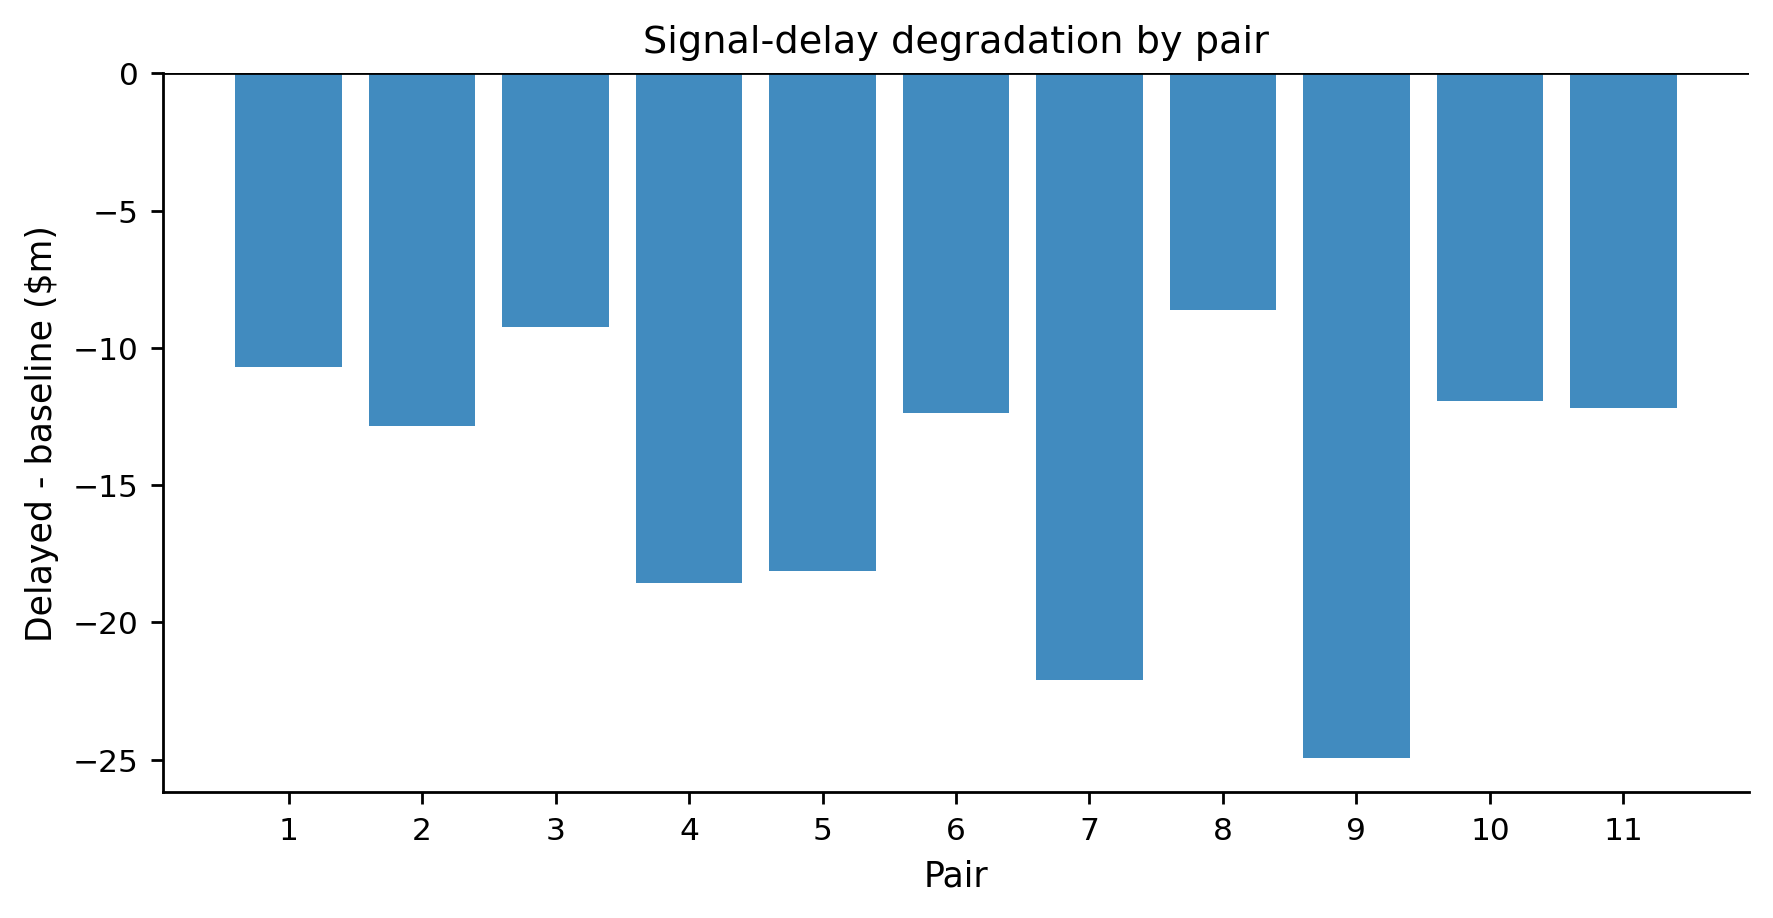
\includegraphics[width=\textwidth]{outputs/presentation_assets/figures/signal_delay_degradation_by_pair.png}
\end{columns}
\vspace{0.2cm}
\small One-minute signal delay materially reduces alpha capture, confirming the short-horizon nature of the signal.
\end{frame}

\begin{frame}{Stress test: forced liquidation}
\begin{columns}[T]
\column{0.58\textwidth}
\scriptsize% Forced liquidation, pair 1
\begin{tabular}{llrllllr}
\hline
Trigger & Mode & Events & Event (\%) & OW PnL ($m) & $\Delta$ ($m) & Cap viol. (\%) & Residual \\
\hline
deterministic_daily & hard_block & 380 & 100.0 & 21.35 & -11.04 & 55.3 & 0 \\
deterministic_daily & capped_with_residual & 380 & 100.0 & 21.88 & -10.52 & 0.0 & 210 \\
probabilistic_daily & hard_block & 33 & 8.7 & 30.64 & -1.76 & 51.5 & 0 \\
probabilistic_daily & capped_with_residual & 33 & 8.7 & 30.62 & -1.77 & 0.0 & 17 \\
\hline
\end{tabular}

\column{0.42\textwidth}
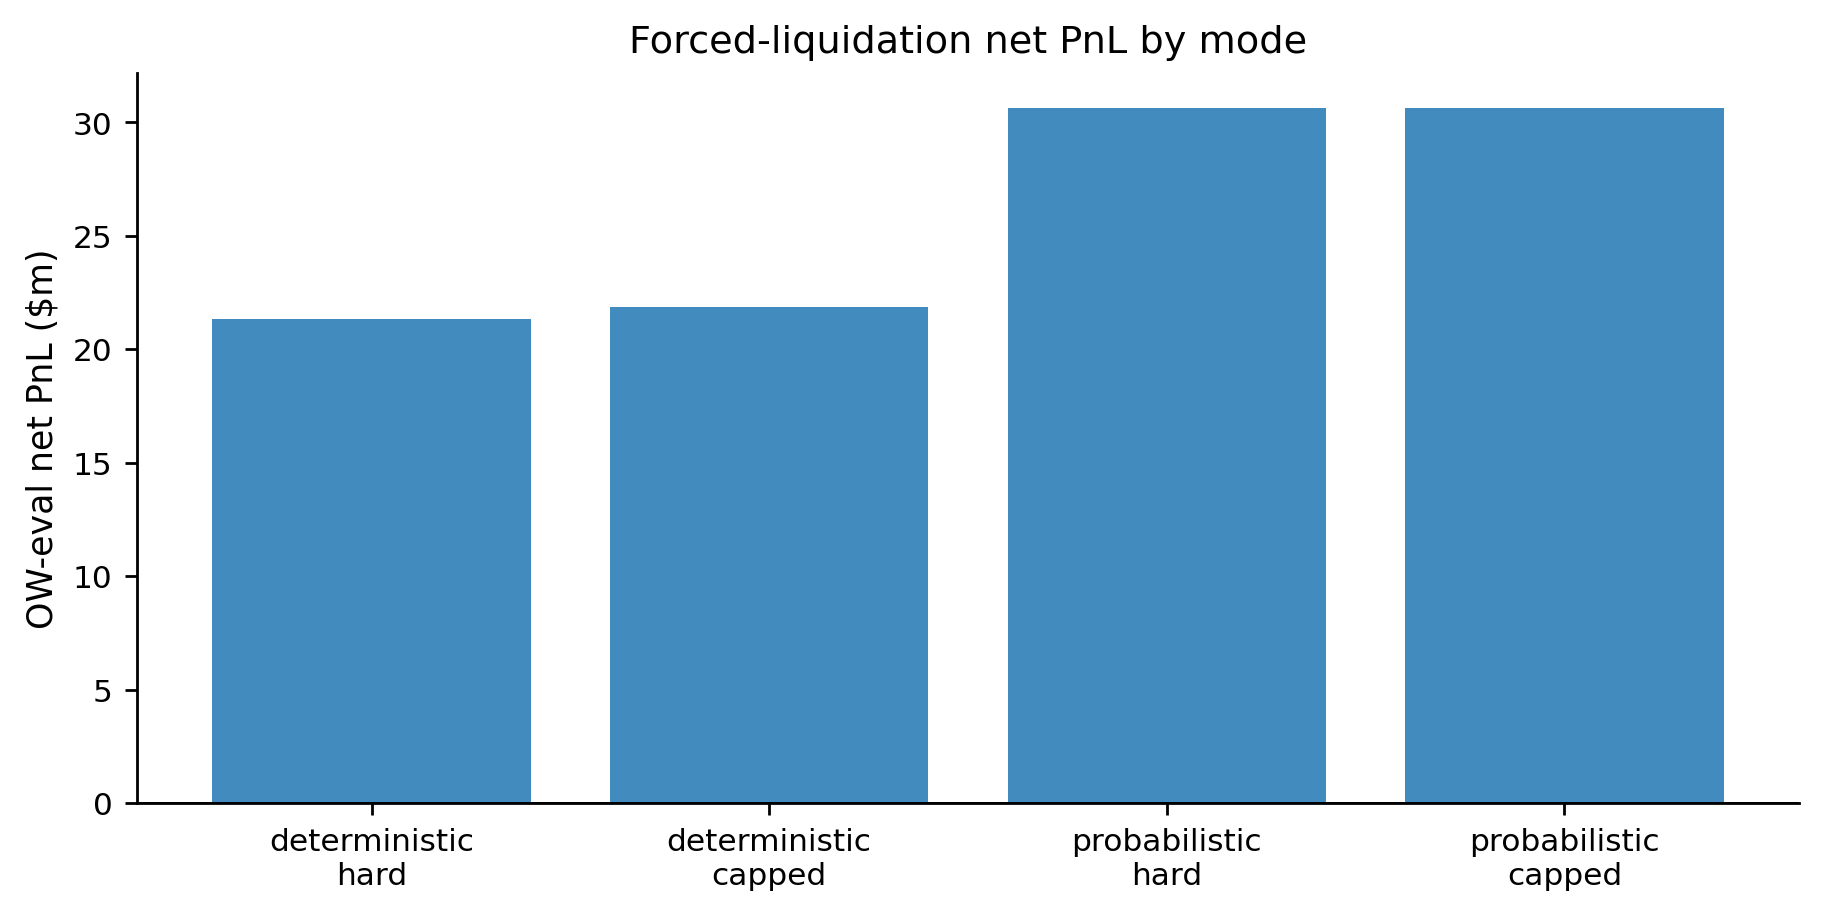
\includegraphics[width=\textwidth]{outputs/presentation_assets/figures/forced_liq_net_pnl_by_mode.png}
\end{columns}
\vspace{0.15cm}
\small Deterministic daily liquidation is a severe systematic shock; probabilistic liquidation is more realistic. Hard block is an upper-bound shock; capped residual is operationally feasible.
\end{frame}

\begin{frame}{Stress test: sizing sensitivity}
\begin{columns}[T]
\column{0.48\textwidth}
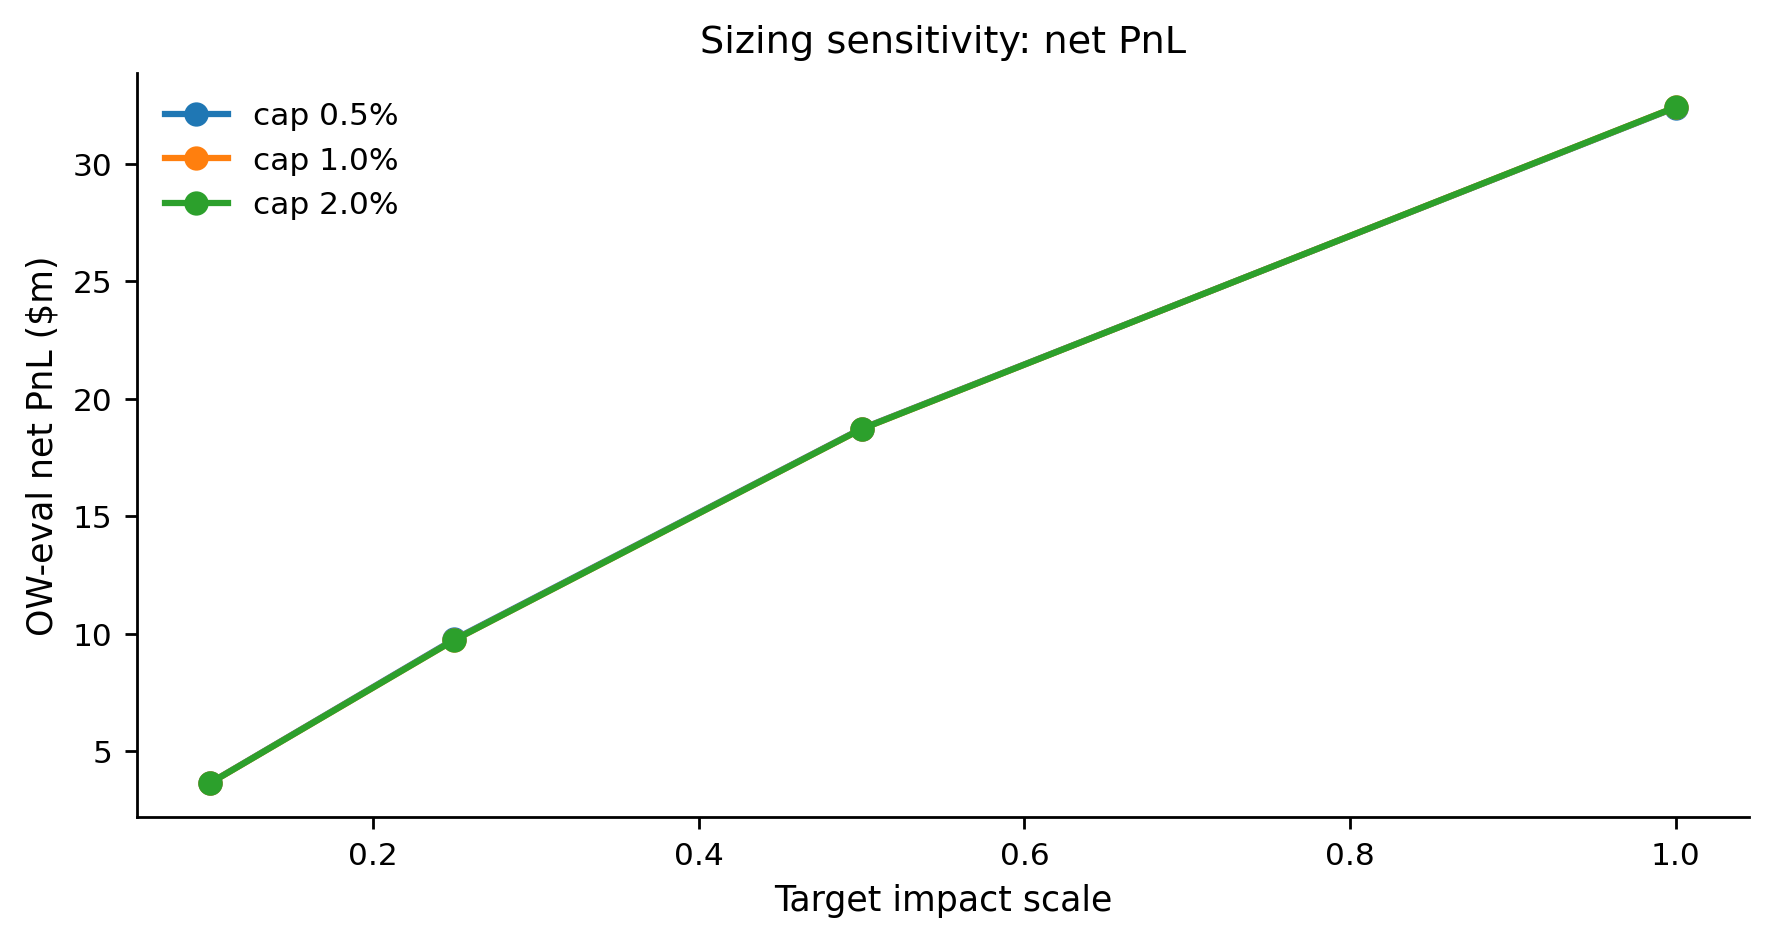
\includegraphics[width=\textwidth]{outputs/presentation_assets/figures/sizing_sensitivity_net_pnl.png}
\column{0.48\textwidth}
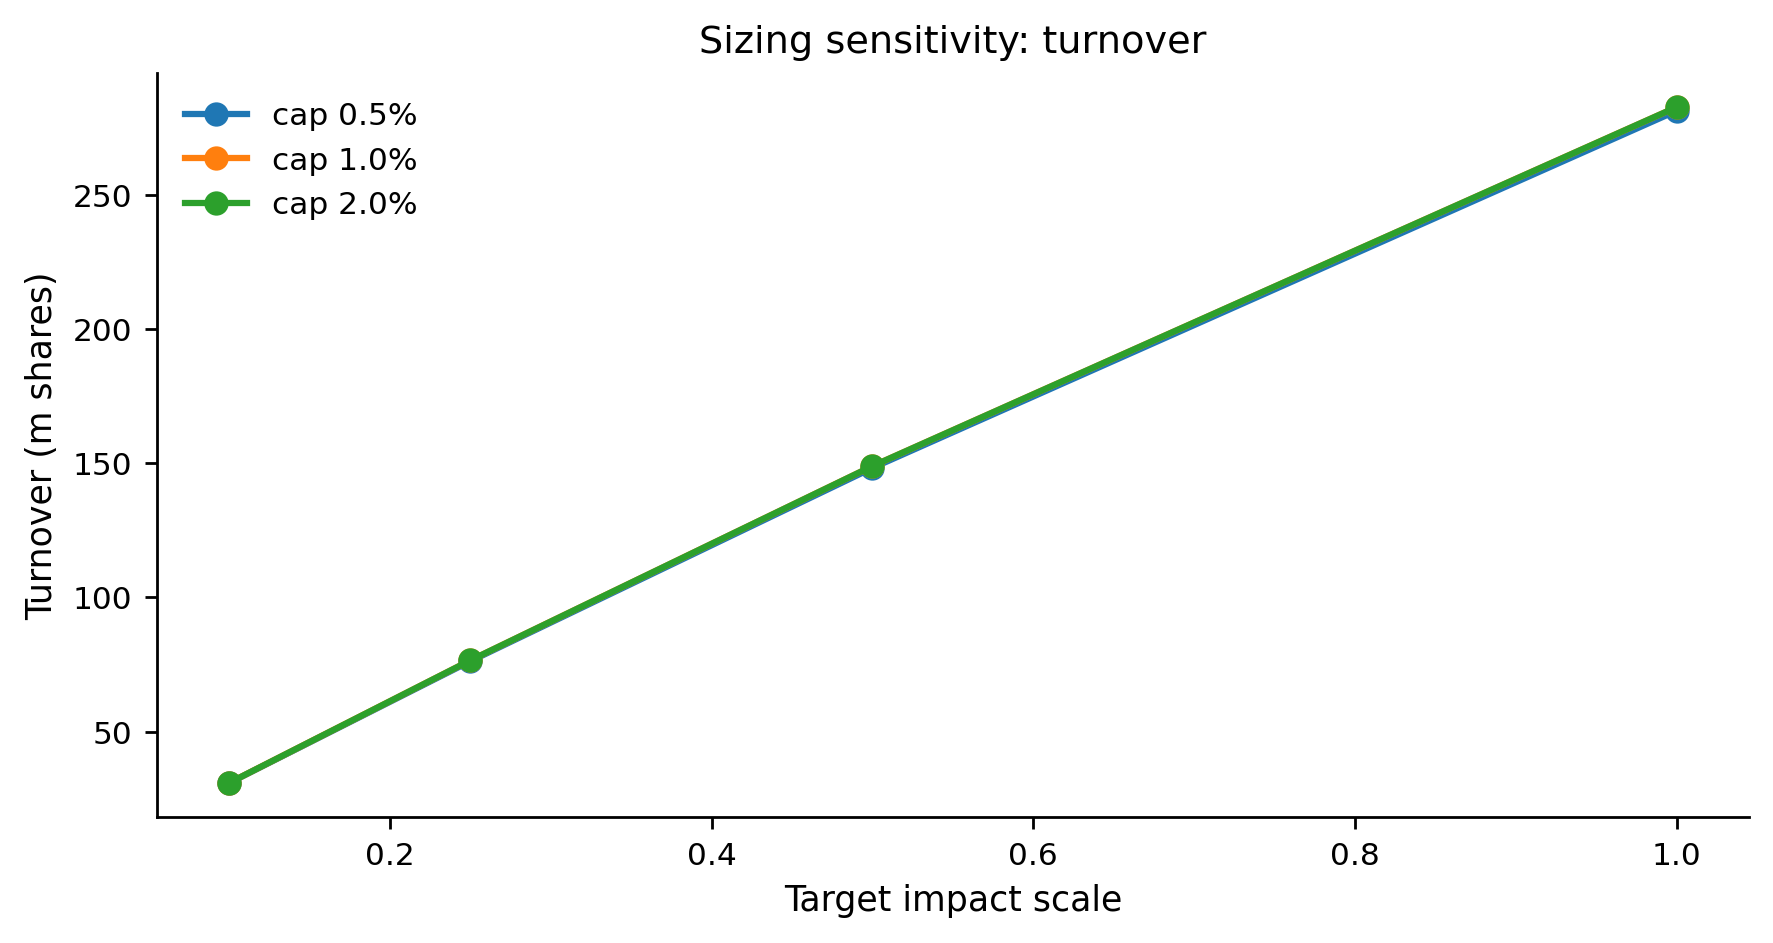
\includegraphics[width=\textwidth]{outputs/presentation_assets/figures/sizing_sensitivity_turnover.png}
\end{columns}
\vspace{0.2cm}
\small Sizing dominates economics: higher participation and target impact increase turnover and may improve gross alpha capture, but also increase impact-cost exposure and clipping.
\end{frame}
